\newcommand{\ypred}{y_{pred}}
\newcommand{\ytrue}{y_{true}}

\section{Theoretical Introduction}

\subsection{Social Homophily}

\epigraph{``People love those who are like themselves.''}{\textit{Rhetoric \\ Aristotle}}

Similarity breeds connection\cite{mcpherson2001birds}. People have several visible characteristics, such as age, gender, and socioeconomic status, for which contact between people with similar properties occurs at a higher rate than between dissimilar people.

There are two overall types of homophily that can be distriguished in groups\cite{lazarsfeld1954}: \textit{status homophily}, in which similarity is based on status, and \textit{value homophily}, which is based on values, attitudes, and beliefs. Status homophily, a part of which is the main study of this thesis, includes the major sociodemographic dimensions that stratify society --- ascribed characteristics like race, ethnicity, sex, or age, and acquired characteristics like religion, education, occupation, and behaviour patterns.

\subsubsection{Age Homophily}

One of the most common homophily patterns in human relations is related to the people's ages\cite{ugander2011}\cite{mcpherson2001birds}. This result is expected because of the many societal reasons that explain the homophily: schools tend to group people according to age into the sane classroooms, work opportunities tend to be clustered into age groups, which affects work environments and neighbourhood composition, and people have a strong tendency to confide in someone of one's own age.

This correlation has a waterfall effect. Since this kind of homophily is present since early into people's life, the producded connections are closer, longer lived, have a larger number of exchanges, and tend to be more personal than other kinds of connections. Indeed, people have a strong tendency to confide in someone of one's own age\cite{mcpherson2001birds}\todo{find better cite}.

There's an interesting exception to this homophily: there is a significant number of connections between parents and their younger children\cite{sarraute2014}\todo{check this}. This exception is addressed later in this paper.

\subsubsection{Gender Homophily}

Lorem ipsum dolor sit amet.

\subsection{Spearman's Coefficient}

Spearman's Rank Correlation Coefficient (also known as Spearman's rho) is a nonparametric measure of rank correlation which measures how well the relationship between two variables can be described using a monotonic function\cite{statistical_analysis}. Unlike Pearson's Correlation Coefficient, which measures lineal relationship between variables, Spearman's Coefficient uses the \emph{rank} of the variables in its calculations; therefore is measures its monotonicity.

For a sample of size \( n \) with scores \( X_i \) and \( Y_i \), the Spearman Coefficient \( r_s \) is defined as

\begin{equation}
r_s = \mathlarger{\rho}_{\rank(X) \rank(Y)} = \frac{\operatorname{cov}(\rank(x), \rank(y))}{\sigma_{\rank(X)} \sigma_{\rank(Y)}}
\label{spearman}
\end{equation}

Where \( \rho_{a,b} \) denotes the Pearson correlation between the variables \( a \) and \( b \). This value will be close to 1 when the variables are directly monotonic, close to -1 when they are inversely monotonic, and close to 0 when there is no tendency for either variable to increase or decrease when the other increases.

\subsection{Bayesian Inference}
This work uses a Bayesian approach to statistics instead of the usual Frequentist approach. In the Frequentist point of view, parameters are fixed and unknown: hypotheses are either true or false, and they cannot be described with a probability. In the Bayesian approach, anything unknown is described with a probability distribution since uncertainty must be described by probability~\cite{mackay}.

The Bayesian approach connects the data \( x \) with a \emph{prior distribution} \( f \left( \theta \right) \) through the \emph{likelihood function} \( f \left( x \middle| \theta \right) \). Instead of estimating the value of \( \hat{\theta} \), the parameter that maximizes the likelihood, Bayesian inference is based on the evaluarion of the \emph{posterior distribution} \( f \left( \theta \middle| x \right) \).

By Bayes Theorem, we can infer the \emph{posterior distribution} using the other parameters.

\begin{equation}
f \left( \theta \mid x \right) = \frac{f \left( x \mid \theta \right) f \left( \theta \right)}{f \left( x \right)}
\label{bayes}
\end{equation}

$f(x)$, the \emph{Marginal Likelihood}, is the probability of observing the data $x$ averaged across the entire space, which acts as a normalizing constant so that the density integrates to 1.

\begin{equation}
f \left( x \right) = \int f \left( x \mid \theta \right) f \left( \theta \right) d \theta
\label{marginal}
\end{equation}

\subsection{Beta Distribution}
\label{subsec:beta}

The \emph{Beta Distribution} is a family of continuos probability distributions defined in the interval $\left[ 0, 1 \right]$ which is parametrized by two shape parameters, $\alpha$ and $\beta$.

The distribution can be used to model the behaviour of \emph{Random Variables} limited to intervals of a finite length. It is often used as a statistical funcion to model unknown data from a known sample, such as allele frequencies in population genetics~\cite{Balding1995}, Malaysian sunshine data~\cite{Sulaiman1999573}, and heterogeneity in the probability of HIV transmission~\cite{SIM:SIM4780080110}.

In the context of \emph{Bayesian Inference}, the \emph{Beta Distribution} is the conjutate prior of the \emph{Binomial Distribution}, which allows us to describe initial knowledge concerning probability of success of a single bi-variate distribution. In layman terms, this allows us to know what is the distribution of the continuous $p$ parameter of a binomial distribution for which we have $\alpha$ positive and $\beta$ negative samples.

\subsubsection{Probability Density Function}

Given a variable $0 \leq x \leq 1$, which represents the unknown probability of having a \emph{Positive Sample} from the distribution, and the shape parameters $\alpha > 0$ and $\beta > 0$, the \emph{Probability Density Function} of the beta distribution can be described as in Equation~\ref{eq:beta_pdf}, where $\kappa$ represents some constant.

\begin{equation}
\label{eq:beta_pdf}
\begin{aligned}
f\left(x; \alpha, \beta\right) &= \kappa \cdot x^{\alpha - 1} {\left( 1 - x \right)}^{\beta - 1} \\
&= \dsfrac{x^{\alpha - 1} {\displaystyle \left( 1 - x \right)}^{\beta - 1}}{\int^1_0 {u^{\alpha - 1} {\left( 1 - u \right)}^{\beta - 1} du}} \\
&= \dsfrac{\Gamma \left( \alpha + \beta \right)}{\Gamma \left( \alpha \right) \Gamma \left( \beta \right)} \cdot x^{\alpha - 1} {\left( 1 - x\right)}^{\beta - 1} \\
&= \dsfrac{1}{\Beta \left(\alpha, \beta\right)} \cdot x^{\alpha - 1} {\left(1 - x\right)}^{\beta - 1}
\end{aligned}
\end{equation}

\begin{equation}
\label{eq:beta_function}
\Beta\left(\alpha, \beta\right) = \frac{\Gamma\left(\alpha + \beta\right)}{\Gamma\left(\alpha\right) \Gamma\left(\beta\right)}
\end{equation}

\Cref{eq:beta_function}, describes the \emph{Beta Function}, which is related to the \emph{Gamma Function} and describes a similar pattern~\cite{thegammafunction}.

Regarding this thesis, the \emph{Beta Distribution} will be used to model a real life problem in Section~\ref{sec:inference_methodology}. In this problem, both $\alpha \in \mathbb{N}$ and $\beta \in \mathbb{N}$, so the \emph{Beta Function} can be simplified using the identity $\left( x - 1 \right)! = \Gamma \left( x \right)$ as shown in Equation~\ref{eq:beta_int}.

\begin{equation}
\label{eq:beta_int}
\Beta(\alpha, \beta) = \frac{(\alpha + \beta - 1)!}{(\alpha - 1)! \cdot (\beta - 1)!}
\end{equation}

Additionally, the \emph{Beta Function} can be generalized into the \emph{Incomplete Beta Function} for some parameter $x$ as in Equation~\ref{eq:incomplete_beta}. This function is, confusingly, also represented with the greek letter $\Beta$; to ease comprehension this thesis will refer to it as $\Betainc$.

\begin{equation}
\label{eq:incomplete_beta}
\Betainc(x; \alpha, \beta) = \int_0^x {t^{\alpha - 1} {(1 - t)}^{\beta - 1} dt}
\end{equation}

As we get more data from the sampling, the \emph{Beta distribution} turns more concenteated towards the actual \( \theta \) and its shapes resembles more a normal curve, as can be seen in \Cref{fig:betagraph}. This represents the increased certainty which comes from the aquired knowledge of the problem.

\begin{figure}
\centering
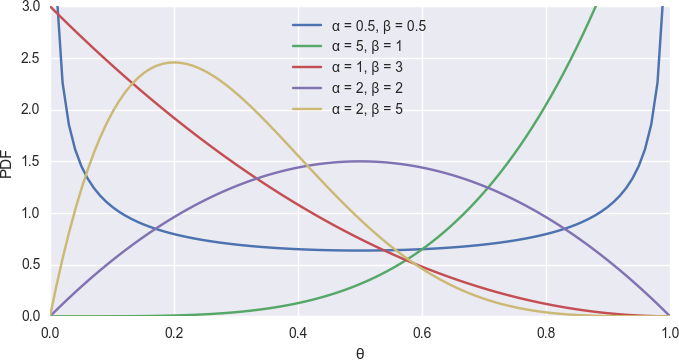
\includegraphics[width=\textwidth]{figures/beta.png}
\caption{Beta distribution with different parameters}
\label{fig:betagraph}
\end{figure}

\subsubsection{Cumulative Distribution Function}

The \emph{Cumulative Distribution Function} of the \emph{Beta Distribution} is defined in Equation~\ref{eq:beta_cdf}.

\begin{equation}
\label{eq:beta_cdf}
\begin{aligned}
F \left( x; \alpha, \beta \right)  &= \int_0^x f \left( t; \alpha, \beta \right) dt \\
&= \int_0^x {\frac{1}{\Beta \left( \alpha, \beta \right)} t^{\alpha - 1} {\left( 1 - t \right)}^{\beta - 1} dt} \\
&= \frac{1}{\Beta \left( \alpha, \beta \right)} \cdot \int_0^x {t^{\alpha - 1} {\left( 1 - t \right)}^{\beta - 1} dt} \\
&= \frac{\Betainc \left( x; \alpha, \beta \right)}{\Beta \left( \alpha, \beta \right)}
\end{aligned}
\end{equation}

$F$ is also known as the \emph{Regularized Incomplete Beta Function}, represented as $I_x(\alpha, \beta)$. This function is related to the \emph{Cumulative Distribution Function} of the \emph{Binomial Distribution}, as shown in Equation~\ref{eq:incomplete_beta_binomial}.

\begin{equation}
\label{eq:incomplete_beta_binomial}
\begin{gathered}
X \sim B \left( n, p \right)  \\
P \left( X \leq k \right)  = I_{1 - p} \left( n - k, k + 1 \right)
\end{gathered}
\end{equation}

\subsection{Machine Learning Validation Metrics}
\label{subsec:mlmetrics}

In the following subsections we present the outline of several supervised machine learning algorithms which are used to compare the Bayesian method to a more realistic baseline. First, we'll present several ways to validate the different algorithms when applied to the data. In the following section, we'll present many of the algorithms used for comparison.

Given a set of fatures $Z$, all of which belong to members of a population which belong to a certain category, and a random subset of those features $X \subseteq Z$ whose category $y$ is known, the models should be trained with $X$ and $y$ in order to correctly predict the values corresponding to all the features in $Z$. Since those values are unknown validation of the output is impossible; therefore, we validate the model using the known values in $X$ and $y$.

There are many metrics that can be used to measure the performance of a classifier or a predictor~\cite{binaryevaluation}; different fields have different preferences due to different goals. In this section, we present many metrics to evaluate different results that are commonly used in the area of mobile phone data analysis~\cite{oskardottir2016}.

\subsubsection{Classification of individual results}

Once we define out classifier $g$ and run it against a matrix\maybe{Set?} of features\maybe{Should I explain train/test split before this subsubsection?}, we get a predicted result $\ypred$ which, when compared to the actual result $\ytrue = y$, can be classified as the one in Table~\ref{tab:confusion}.

\begin{table}[h]
\begin{tabularx}{\textwidth}{| c | X | X X |}
\hline

& & \multicolumn{2}{c|}{\textbf{Predicted Condition}} \\
& Total Population &
\makecell{Condition Positive} &
\makecell{Condition Negative} \\ \hline

\multirow{2}{5em}{\textbf{True Condition}} &
Condition Positive &
\cellcolor{OrangeRed} \makecell{\textbf{True Positive}} &
\cellcolor{CadetBlue} \makecell{\textbf{False Negative} \\ (Type II error)} \\


& Condition Negative &
\cellcolor{CadetBlue} \makecell{\textbf{False Positive} \\ (Type I Error)} &
\cellcolor{OrangeRed} \makecell{\textbf{True Negative}} \\ \hline

\end{tabularx}
\caption[caption]{Confusion Table, showing different classifications of an individual prediction. \\ True and False Positives ($\TP$/$\FP$) refer to the number of predicted positives that were correct/incorrect, and similarly for True and False Negatives ($\TN$/$\FN$).}
\label{tab:confusion}
\end{table}

Additionally, this table can be easily seen in a graphical way in figure~\ref{fig:truefalsenegativepositive}.

\begin{figure}
\centering
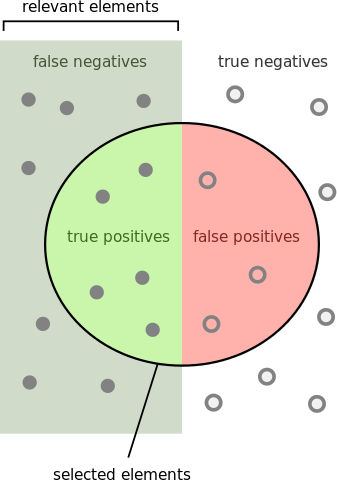
\includegraphics[width=15em]{figures/TrueFalseNegativePositive.png}
\caption{Visual explanation of \emph{Precision} and \emph{Recall}}
\label{fig:truefalsenegativepositiv}
\end{figure}

\subsubsection{Precision and Recall}
\label{subsec:precisionrecall}
\emph{Precision} denotes the proportion of predicted positive cases that are correctly real positive. Trying to maximize this would allow us to adjust a particular predictor so that the majority of the predicted cases are actually positive. Conversely, \emph{recall} is the proportion of real positive cases that are correctly predicted positive, and maximizing it would allow us to adjust a predictor so that the majority of positive cases are predicted.

\begin{equation}
\begin{split}
\Precision = \TPA &= \frac{\TP}{\TP + \FP} \\
\Recall = \TPR &= \frac{\TP}{\TP + \FN}
\end{split}
\label{precisionrecall}
\end{equation}

These two measures and their combinations focus only on the positive examples and predictions, althrough between them they capture some information about the rates and kind of errors made\cite{binaryevaluation}. While the \emph{recall} has been shown to have a major weight in working with machine translation\cite{fraser2007}, they aren't particularly useful to use alone since they don't take into account many factors of the prediction\cite{binaryevaluation}.

\subsubsection{Inverse~Precision and Inverse~Recall}

As a corollary of the previous metrics, we can add metrics that measure the proportion of real negative cases that are correctly predicted negative, referred as the \emph{Inverse~Recall}, and the proportion of predicted negatives that are real negatives, referreed as the \emph{Inverse~Precision}\cite{binaryevaluation}. We can see that these are equivalent to finding the \emph{Precision} and \emph{Recall} of the negative category.

\begin{equation}
\begin{split}
\InvPrecision = \TNR &= \frac{\TN}{\FP + \TN} \\
\InvRecall = \TNA &= \frac{\TN}{\FN + \TN}
\end{split}
\label{negativeprecisionrecall}
\end{equation}

\subsubsection{Accuracy}
\label{subsec:accuracy}
The \emph{accuracy}, commonly referred in te context of binary classifiers as \textbf{Rand~Accuracy}\cite{powers15}, is used as a statistical measure of how well a binary classification test identifies or excludes a condition. Unlike the \emph{precision}, it takes into account the negatives, and it's expressible\cite{binaryevaluation} both as a weighted average of \emph{precision} and inverse \emph{precision} or \emph{recall} and \emph{inverse recall}.

\begin{equation}
\Accuracy = \frac{\TP + \TN}{N}
\label{accuracy}
\end{equation}

This can be more simply expressed using the weighted average of either the \emph{Precision} and \emph{Inverse~Precision} or the \emph{Recall} and the \emph{Inverse~Recall}.

\begin{equation}
\begin{split}
\Accuracy &= \left(\TP + \TN\right) \cdot \TPR + \left(\FP + \TN\right) \cdot \TNR \\
&= \left(\TP + \FP\right) \cdot \TPA + \left(\FN + \TN\right) \cdot \TNA
\end{split}
\label{accuracy2}
\end{equation}

\subsubsection{ROC Curve}

A \emph{Receiver Operating Characteristing} graph is a technique for visualizing, organizing, and selecting classifiers based on their performance\cite{fawcett2005}. The curve is created by plotting the \emph{True Positive Rate} against the \emph{False Positive Rate} at various threshold settings.

This allows to compare different classifiers before having to select a particular threshold value for them. In particular, a random classifier will score near the positive diagonal ($\FPR = \TPR$), while a perfect classifier will score in the top left hand corner ($\FPR = 1, \TPR = 0$) and a worst case classifier will score in the bottom right hand corner\footnote{Note that, for any binary classifier, it's trivial to transpose the entire ROC curve (or a part of it) to the other part of the diagonal; therefore the worst ``realistic'' case is the random one}\cite{binaryevaluation}.

\begin{figure}
\todo{Add figure of ROC with AUC}
\caption{A \emph{ROC Curve}, where the \emph{Area Under the Curve} is marked}
\label{fig:roc}
\end{figure}

\subsubsection{Area Under the Curve}
\label{subsec:auc}
The \emph{ROC Curve} allows us to compare classifiers and choose the one which is closer to optimal in some sense. While there are many possible parametrizations, the most common is to minimize the \emph{Area Under the Curve}, which is equal to the probability that a classifier will rank a randomly chosen positive instance higher than a randomly chosen negative one\cite{fawcett2005}. This can be formulated as shown in formula~\ref{eq:auc}.

\begin{equation}
\begin{split}
\AUC &= P\left(X_1 > X_0\right) \\
&= \todo{Something something}
\end{split}
\label{eq:auc}
\end{equation}

\subsubsection{F-measure}
\label{subsec:fmeasure}
The \emph{F-measure} is another measure of a tests accuracy. It considers both the \emph{Precision} and the \emph{Recall} of the test to compute the score. It can be considered the weighted average of both values for some weight $\beta$, where $F_\beta$ reaches the best score 1 when both precision and recall are 1.

\begin{equation}
\begin{split}
F_\beta &= \left( 1 + \beta^2 \right) \cdot \frac{\TPA \cdot \TPR}{\left( \beta^2 \cdot \TPA \right) + \TPR} \\
&= \frac{\left( 1 + \beta^2 \right) \cdot \TP}{\left( 1 + \beta^2 \right) \cdot \TP + \beta^2 \cdot \FN + \FP}
\end{split}
\end{equation}

The most commonly used \emph{F-measure}, $F_1$, measures the \emph{Precision} and \emph{Recall} is thet harmonic mean of the \emph{Precision} and \emph{Recall}. In particular, for an \emph{F-measure} with $\beta > 1$ weights Recall higher than Precision, while with $beta < 1$ weights Precision higher than Recall.

\subsection{Supervised Machine Learning Models}

This section presents several \emph{Supervised Machine Learning} models that are used in the paper. All models work using the process described in the introduction to Section~\ref{sucsec:mlmetrics} with a 

\subsubsection{Logistic Regression}
\label{subsec:logisticregression}

\subsubsection{Decision Trees}
\label{subsec:decisiontrees}
\todo{Describe Decision Trees}

\subsubsection{Random Forest}
\label{subsec:randomforest}
\todo{Add Random Forest}

